\scanpage{53}
\[
\text{(62)}\qquad(M_{[G]},\Gamma^!)\simeq B(\Gamma^!_{S_0})
\]
La ``dimension modulaire \inserted{ambiante}'' d'un tel $\underline G$ est égale à :
\deleted{$\unsure{3(h_1(G)-1)+\nu}$ \quad $\unsure{\nu}=\operatorname{card}I$}
\[
\text{(63)}\qquad\dim\operatorname{tot}(G)=3(g-1)+\underset{\substack{\Vert\\\operatorname{card}I}}{\nu}=3(h_1(G)-1)+\nu.
\]
\margin{puisque $g=\underbrace{\sum_\alpha g_\alpha}_{0}+h_1$}
Nous allons faire l'énumération des cas où cette dimension est $\leq2$, ce qui implique déjà $h_1\leq1$, i.e. $h_1\in\{0,1\}$.

\deleted{a) $\unsure{\dim\operatorname{tot}(G)}=0$}

a) $h_1=0$ i.e. $G$ est un \uline{arbre}, la dim. modulaire est $\nu-3$, donc on doit avoir $\nu\geq3$. Si on veut que cette dim soit $\leq\unsure{2}$, cela signifie que $3\leq\nu\leq5$.

Un arbre qui n'est pas réduit à un \deleted{\unsure{arbre}} sommet, ni à un segment, a au moins trois bouts, dont chacun doit avoir un poids marqué $\geq2$, donc $\nu\geq6$ --- donc si $\nu\leq5$, on voit que l'arbre est un sommet, ou un segment. On trouve les cas
\figure{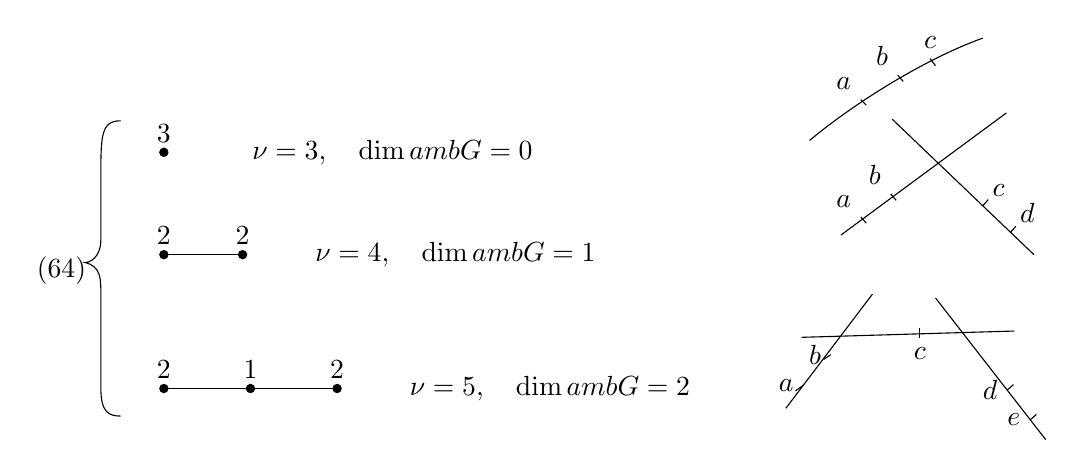
\begin{tikzpicture}[x=1cm,y=1cm]
\node at (-1.3,-1.5) {$(64)$};
\draw (-.55,.4) .. controls (-.8,.4) and (-.8,.2) .. (-.8,-.3) -- (-.8,-1.1) .. controls (-.8,-1.35) and (-.95,-1.4) .. (-1,-1.4) .. controls (-.8,-1.45) and (-.8,-1.6) .. (-.8,-1.8) -- (-.8,-3.0) .. controls (-.8,-3.3) and (-.7,-3.35) .. (-.55,-3.35);
\fill (0,0) circle (1.7pt); \node[above] at (0,0) {$3$};
\node[right] at (1,0) {$\nu=3,\quad\dim\operatorname{amb}G=0$};
\draw (0,-1.3)--(1,-1.3); \fill (0,-1.3) circle (1.7pt); \fill (1,-1.3) circle (1.7pt);\node[above] at (0,-1.3) {$2$};\node[above] at (1,-1.3) {$2$};
\node[right] at (1.8,-1.3) {$\nu=4,\quad\dim\operatorname{amb}G=1$};
\draw (0,-3)--(2.2,-3);\fill (0,-3) circle (1.7pt);\fill (1.1,-3) circle (1.7pt);\fill (2.2,-3) circle (1.7pt);
\node[above] at (0,-3) {$2$};\node[above] at (1.1,-3) {$1$};\node[above] at (2.2,-3) {$2$};\node[right] at (3,-3) {$\nu=5,\quad\dim\operatorname{amb}G=2$};
\draw (8.2,.15) .. controls (8.8,.65) and (9.7,1.2) .. (10.4,1.45);
\draw (8.85,.67)--(8.92,.60);\node[above left] at (8.85,.67) {$a$};\draw (9.32,.98)--(9.39,.90);\node[above left] at (9.32,.98) {$b$};\draw (9.73,1.19)--(9.80,1.10);\node[above] at (9.73,1.19) {$c$};
\draw (8.6,-1.05)--(10.7,.5);\draw (9.25,.42)--(11.05,-1.3);
\draw (8.85,-.82)--(8.92,-.9);\node[above left] at (8.85,-.82) {$a$};\draw (9.23,-.53)--(9.30,-.61);\node[above left] at (9.23,-.53) {$b$};\draw (10.4,-.68)--(10.47,-.60);\node[above right] at (10.4,-.68) {$c$};\draw (10.75,-1.02)--(10.82,-.94);\node[above right] at (10.75,-1.02) {$d$};
\draw (8.1,-2.35)--(10.8,-2.27);\draw (7.9,-3.25)--(9,-1.8);\draw (9.8,-1.85)--(11.2,-3.65);
\draw (8.12,-2.96)--(8.02,-3.03);\node[left] at (8.12,-2.96) {$a$};\draw (8.47,-2.57)--(8.38,-2.63);\node[left] at (8.47,-2.57) {$b$};\draw (9.6,-2.36)--(9.6,-2.23);\node[below] at (9.6,-2.36) {$c$};\draw (10.71,-3.02)--(10.79,-2.95);\node[left] at (10.71,-3.02) {$d$};\draw (11.0,-3.4)--(11.08,-3.33);\node[left] at (11,-3.4) {$e$};
\end{tikzpicture}}
\margin{52}
